%%%%%%%%%%%%%%%%%%%%%%%%%%%%%%%%%%%%%%%%%
% Beamer Presentation
% LaTeX Template
% Version 1.0 (10/11/12)
%
% This template has been downloaded from:
% http://www.LaTeXTemplates.com
%
% License:
% CC BY-NC-SA 3.0 (http://creativecommons.org/licenses/by-nc-sa/3.0/)
%
%%%%%%%%%%%%%%%%%%%%%%%%%%%%%%%%%%%%%%%%%

%----------------------------------------------------------------------------------------
%	PACKAGES AND THEMES
%----------------------------------------------------------------------------------------

\documentclass{beamer}

\mode<presentation> {

% The Beamer class comes with a number of default slide themes
% which change the colors and layouts of slides. Below this is a list
% of all the themes, uncomment each in turn to see what they look like.

%\usetheme{default}
%\usetheme{AnnArbor}
%\usetheme{Antibes}
%\usetheme{Bergen}
\usetheme{Berkeley}
%\usetheme{Berlin}
%\usetheme{Boadilla}
%\usetheme{CambridgeUS}
%\usetheme{Copenhagen}
%\usetheme{Darmstadt}
%\usetheme{Dresden}
%\usetheme{Frankfurt}
%\usetheme{Goettingen}
%\usetheme{Hannover}
%\usetheme{Ilmenau}
%\usetheme{JuanLesPins}
%\usetheme{Luebeck}
%\usetheme{Madrid}
%\usetheme{Malmoe}
%\usetheme{Marburg}
%\usetheme{Montpellier}
%\usetheme{PaloAlto}
%\usetheme{Pittsburgh}
%\usetheme{Rochester}
%\usetheme{Singapore}
%\usetheme{Szeged}
%\usetheme{Warsaw}

% As well as themes, the Beamer class has a number of color themes
% for any slide theme. Uncomment each of these in turn to see how it
% changes the colors of your current slide theme.

%\usecolortheme{albatross}
%\usecolortheme{beaver}
%\usecolortheme{beetle}
%\usecolortheme{crane}
%\usecolortheme{dolphin}
%\usecolortheme{dove}
%\usecolortheme{fly}
\usecolortheme{lily}
%\usecolortheme{orchid}
%\usecolortheme{rose}
%\usecolortheme{seagull}
%\usecolortheme{seahorse}
%\usecolortheme{whale}
%\usecolortheme{wolverine}

%\setbeamertemplate{footline} % To remove the footer line in all slides uncomment this line
%\setbeamertemplate{footline}[page number] % To replace the footer line in all slides with a simple slide count uncomment this line

%\setbeamertemplate{navigation symbols}{} % To remove the navigation symbols from the bottom of all slides uncomment this line
}
\usepackage{graphicx} % Allows including images
\usepackage{booktabs} % Allows the use of \toprule, \midrule and \bottomrule in tables

\usepackage{amsmath}
\usepackage{amssymb}
\usepackage{mathptmx}
\usepackage[framemethod=tikz]{mdframed}
\usepackage{bm}
\DeclareSymbolFontAlphabet{\mathnormal}{letters}

\setbeamercolor{upcol}{fg=black,bg=yellow}
\setbeamercolor{lowcol}{fg=black,bg=yellow!40}


%----------------------------------------------------------------------------------------
%	TITLE PAGE
%----------------------------------------------------------------------------------------

\title[Short title]{Weekly Summary} % The short title appears at the bottom of every slide, the full title is only on the title page

\author{Shiqi Duan} % Your name
\institute[USTC] % Your institution as it will appear on the bottom of every slide, may be shorthand to save space
{
University of Science and Technology of China \\ % Your institution for the title page
\medskip
\textit{sqduan@mail.ustc.edu.cn} % Your email address
}
\date{\today} % Date, can be changed to a custom date

\begin{document}

\begin{frame}
\titlepage % Print the title page as the first slide
\end{frame}

\begin{frame}
\frametitle{Overview} % Table of contents slide, comment this block out to remove it
\tableofcontents % Throughout your presentation, if you choose to use \section{} and \subsection{} commands, these will automatically be printed on this slide as an overview of your presentation
\end{frame}

%----------------------------------------------------------------------------------------
%	PRESENTATION SLIDES
%----------------------------------------------------------------------------------------

%------------------------------------------------
\section{Kalman filter}
 % Sections can be created in order to organize your presentation into discrete blocks, all sections and subsections are automatically printed in the table of contents as an overview of the talk
%------------------------------------------------



%------------------------------------------------


%------------------------------------------------

\begin{frame}
\frametitle{Kalman filter Review}
\begin{block}{What is a kalman filter}
	
The kalman filter is an estimator for what is called the linear quadratic estimator.
 
Used for estimating dynamic process perturbed by white noise.

\begin{itemize}
	\item It's a mathematical tool 
	\item It's a program 
	\item It's a consistent statistical characterization of an estimation problem
	
\end{itemize}

\end{block}

\end{frame}

\begin{frame}
\frametitle{Mathematical form}
\begin{block}{Estimation ("Predict with prior knowledge")}

\begin{equation}
\begin{aligned} \hat{\mathbf{x}}_{k | k-1} &=\mathbf{F}_{k} \hat{\mathbf{x}}_{k-1 | k-1}+\mathbf{B}_{k} \mathbf{u}_{k}\\ \mathbf{P}_{k | k-1} &=\mathbf{F}_{k} \mathbf{P}_{k-1 | k-1} \mathbf{F}_{k}^{T}+\mathbf{Q}_{k} \end{aligned}
\end{equation}

\end{block}

\begin{block}{Update based on measurement ("Correct")}

First we calculate the gains
\begin{equation}
\begin{array}{l}{\tilde{\mathbf{y}}_{k}=\mathbf{z}_{k}-\mathbf{H}_{k} \hat{\mathbf{x}}_{k | k-1} } \\ {\mathbf{S}_{k}=\mathbf{H}_{k} \mathbf{P}_{k | k-1} \mathbf{H}_{k}^{T}+\mathbf{R}_{k}} \\ {\mathbf{K}_{k}=\mathbf{P}_{k | k-1} \mathbf{H}_{k}^{T} \mathbf{S}_{k}^{-1}}\end{array}
\end{equation}

$\tilde{\mathbf{y}}_{k}$ is the measurement residual; $\mathbf{S}_{k}$ is the covariance matrix of measurement residual; $\mathbf{K}_{k}$ is the optimal Kalman gain
\end{block}

\end{frame}

\begin{frame}
\frametitle{Mathematical form}
Then we use them to update variable $\mathbf{x}$ and $\mathbf{P}$

\begin{equation}
\begin{aligned} \hat{\mathbf{x}}_{k | k} &=\hat{\mathbf{x}}_{k | k-1}+\mathbf{K}_{k} \tilde{\mathbf{y}}_{k}\\ \mathbf{P}_{k | k} &=\left(I-\mathbf{K}_{k} \mathbf{H}_{k}\right) \mathbf{P}_{k | k-1} \end{aligned}
\end{equation}

\end{frame}
%------------------------------------------------


%------------------------------------------------
\section{Learn MPC (1) -- what and why}

\begin{frame}
\frametitle{Main components}


\begin{itemize}
	\item Prediction
	\item Receding horizon
	\item Modelling
	\item Performance index
	\item Degree of freedom
	\item Constraint handling
	\item Multivariable
\end{itemize}

\end{frame}

\begin{frame}
\frametitle{Main components}
\begin{block}{Prediction}
	
	Prediction horizen $>$ settling time
\end{block}

\begin{block}{Prediction}
	
	Continually update our predictions and decision making using the most recent target and measurement data.
\end{block}

\begin{block}{Modelling}
	
	The simplest model gives accurate prediction is usually the best.
\end{block}

\end{frame}

\begin{frame}
\frametitle{Main components}
\begin{block}{Performance index}
	
\end{block}

\begin{itemize}
	\item What is the performance index for?
	
	The performance index is a numerical definition of what is the best.
	
	\item How to design the performance index?
	
	One should only increase the complexity where the benefits is clear.
\end{itemize}


\begin{figure}
	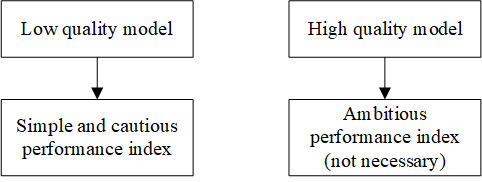
\includegraphics[width=0.7\linewidth]{Figures/lowandhigh}
\end{figure}


\end{frame}

\begin{frame}
\frametitle{Main components}

Typically quadratic performance is used, because:

\begin{enumerate}
	\item It give us well conditioned optimization
	
	\item Unique minimum
	
	\item Smooth behaviours (unlike 1-norm or inf-norm)
\end{enumerate}

\begin{itemize}
	\item How to balance optimal and robust performance?

\end{itemize}

\begin{figure}
	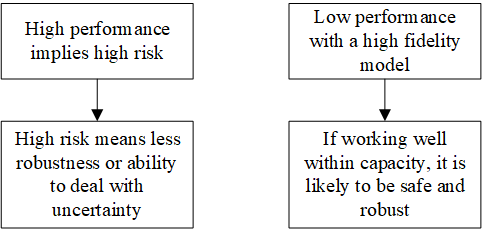
\includegraphics[width=0.7\linewidth]{Figures/lowandhigh1}
\end{figure}

\end{frame}

\begin{frame}
\frametitle{Main components}

\begin{block}{Degree of freedom}

\end{block}
The useful num of DOF is related to the prediction accuracy. 
\medskip

In MPC, an ill-posed performance index means \textbf{a low prediction horizon compared to the system dynamic and use numerous DOF to optimal tracking with that horizon.}
\medskip

\begin{beamerboxesrounded}[upper=upcol,lower=lowcol,shadow=true]
	 
	The useful num of DOF is related to the prediction accuracy
\end{beamerboxesrounded}


\end{frame}

\begin{frame}
\frametitle{Main components}
\begin{block}{Constraint handling}
	
\end{block}

One major advantage of MPC is it \textbf{embeds constraints to strategy}, which means that it will not propose input flows that allow overshooting, the response time may become slower, but much more safer.

\end{frame}

\begin{frame}
\frametitle{Why we use MPC}

\begin{itemize}
	\item Intuitive concept, easy to understand and implement
\item	Systematic handling of constrains
\item	Can handle MIMO and dead-time without modification
\item	Feed forward to make good use of future target information
\item	Handling challenging dynamics (unlike PID)
\end{itemize}

\end{frame}



\section{Learn MPC (2) - Modelling}

\begin{frame}
\frametitle{Model requirements}

\begin{block}{Simple model?}

Simple manipulation and algebra requires linear models. If these are good enough, \textbf{use linear models in MPC}.

\end{block}

\begin{block}{Discrete or continuous?}
	
Decision making requires processing time, there for, \textbf{MPC laws are implemented in discrete time}.
	
\end{block}

\end{frame}

\begin{frame}
\frametitle{Model requirements}

\begin{block}{What sample rate?}
	
	A typical argument is that one wants around \textbf{10 sample points} within a typical response (settling time or rise time)
	
	\begin{figure}
		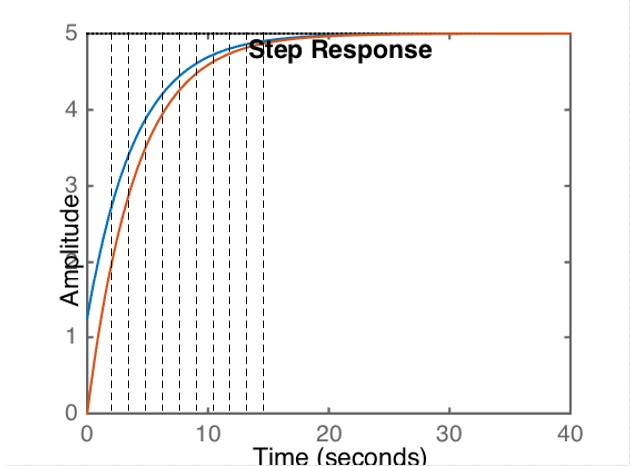
\includegraphics[width=0.6\linewidth]{Figures/sampling_time}
	\end{figure}
	
\end{block}

\end{frame}


\begin{frame}
\frametitle{Modelling}

\begin{block}{Model form}
	\begin{itemize}
		\item State space model
		\item	Transfer function model
		\item	Step response model
		\item	Independent model
	\end{itemize}
\end{block}



\end{frame}

\section{Prediction}
\label{lqr}

\subsection{Prediction with SS model}

\begin{frame}
\frametitle{Basic concepts of prediction}

Given data at time $k$, we can determine the data at $k+1$

\begin{equation}
\left.\begin{array}{rl}{x_{k+1}} & {=A x_{k}+B u_{k}} \\ {y_{k}} & {=C x_{k}+d_{k}}\end{array}\right\} \Rightarrow \begin{array}{c}{y_{k+1}=C x_{k+1}+d_{k+1}} \\ {y_{k+1}=C A x_{k}+C B u_{k}+d_{k+1}}\end{array}
\end{equation}

Nomally we can assume that $d_k=d_{k+1}$.

\end{frame}

\begin{frame}
\frametitle{Basic concepts of prediction}

\begin{block}{Splitting predictions}
	We can saperate the predictions into known and unknown part
	
	
\end{block}
\begin{equation}
	\begin{split}
		y_{k+n| k}=&C A^{n} x_{k}+d_{k}+\\
		&C\left(A^{n-1} B u_{k |k}+A^{n-2} B u_{k+1 |k}+\cdots+B u_{k+n-1| k}\right)
	\end{split}
\end{equation}

\begin{itemize}
\item known: $C A^{n} x_{k}+d_{k}$, based on current and past measurement

\item unknown: $C\left(A^{n-1} B u_{k |k}+A^{n-2} B u_{k+1 |k}+\cdots+B u_{k+n-1| k}\right)$, based on future input choices.
\end{itemize}
\end{frame}


\begin{frame}
\frametitle{Matrix form of ss prediction}

Rewrite the prediction in matrix form:

\begin{small} 
\begin{equation}
\mathbf{x}_{k+1} =
\left[
\begin{array}{c}{A \textbf{x}_{k}} 
\\ {A^{2} \textbf{x}_{k}} 
\\ {\vdots} 
\\ A^{n} \textbf{x}_k\end{array}\right]
+\left[\begin{array}{c}{B u_{k |k}} 
\\ {A B u_{k| k}+B u_{k+1| k}} \\ {\vdots} \\ {A^{n-1} B u_{k| k}+\cdots+A B u_{k+n-2| k}+B u_{k+n-1 |k}}\end{array}\right]
\end{equation}
\end{small}

make seperation, we get

\begin{small}
	\begin{equation}
	\textbf{x}_{k+1}=\left[\begin{array}{c}{A} \\ {A^{2}} \\ {\vdots} \\ {A^{n}}\end{array}\right] \textbf{x}_{k}+\left[\begin{array}{cccc}{B} & {0} & {\cdots} & {0} \\ {A B} & {B} & {\cdots} & {0} \\ {\vdots} & {\vdots} & {\ddots} & {\vdots} \\ {A^{n-1} B} & {A^{n-2} B} & {\cdots} & {B}\end{array}\right]\left[\begin{array}{c}{u_{k| k}} \\ {u_{k+1 |k}} \\ {\vdots} \\ {u_{k+n-1 |k}}\end{array}\right]
	\end{equation}
\end{small}

\end{frame}

\begin{frame}
\frametitle{Matrix form of ss prediction}

\begin{itemize}
	\item State prediction
	\begin{equation}
	\textbf{x}_{k+1}=P_{x} \textbf{x}_{k}+H_{x} \textbf{u}_{k}
	\end{equation}
	
	\item Output predictions
	\begin{equation}
	\textbf{y}_{k+1}=P \textbf{x}_{k}+L d_{k}+H \textbf{u}_{k}
	\end{equation}
\end{itemize}

\end{frame}

\begin{frame}
\frametitle{Unfinished Work}
\begin{itemize}
	\item Try to design a kalman filter for the LQG problem
	\item Continue on MPC and design a simple MPC demo
\end{itemize}

\end{frame}
%------------------------------------------------



%------------------------------------------------




%------------------------------------------------


%------------------------------------------------


%------------------------------------------------


%------------------------------------------------


\begin{frame}
\frametitle{References}
\footnotesize{
\begin{thebibliography}{99} % Beamer does not support BibTeX so references must be inserted manually as below
\bibitem[Mohinder S. Grewal, 2014]{p1} Mohinder S. Grewal (2014)
\newblock Kalman Filtering: Theory and Practice Using MATLAB
\newblock \emph{ Wiley-IEEE Press} 
\end{thebibliography}

\begin{thebibliography}{100} % Beamer does not support BibTeX so references must be inserted manually as below
	\bibitem[Welch G, 1995]{p1} Welch G (1995)
	\newblock An introduction to the Kalman filter
	\newblock \emph{Journal} 
\end{thebibliography}
}
\end{frame}

%------------------------------------------------

%----------------------------------------------------------------------------------------

\end{document} 